\newpage
\section{리눅스 커널에 적용}
\label{sec:linux}

%\subsection{Reverse mapping}

%$$$$$$$$$$$$$$$$$$$$$$$$$$$$$$$$$$$$$$$$$$$$$$$$$$$$$$$$$$$$$$$$$$$$$$$$$$$$$$$$
%Paragraph 1: Linux의 reverse mapping에 대한 자세한 설명 
%$$$$$$$$$$$$$$$$$$$$$$$$$$$$$$$$$$$$$$$$$$$$$$$$$$$$$$$$$$$$$$$$$$$$$$$$$$$$$$$$

%This section shows how to apply the \LDU to the complex Linux
%virtual memory system 
이번 장은 리눅스 커널의 업데이트 직렬화에 대한 문제를 풀기 위해,
우리가 어떻게 LUD를 복잡한 리눅스 가상 메모리 시스템에 적용했는지에 대해 설명한다.
이번 장은 더욱 현실적인 내용을 다룬다.
%to solve the update serialization problem;it deals with more practical one.

%The Linux reverse page mapping(rmap), a kernel memory management mechanism,
% consists of anonymous rmap and file rmap, are a update-heavy data structure.
리눅스 역 매핑(rmap)은 커널 메모리 관리 메커니즘(mechanism) 중 하나이다.
이것은 익명 역 매핑과 파일 역 매핑으로 구성되며 이것은 업데이트 비율이 높은 자료구조이다.
%These two rmaps maintain virtual address(VMAs) to translate physical
%addresses to virtual address~\cite{Dave2004OLSRMAP}, and the rmaps are a shared
% global resource between processes.
이러한 두가지 rmap은 리눅스의 가상 주소(VMAs)를 관리하고, 이것은 물지 주소(physical address)를 
가상 주소로 변환하는 일을 하며, rmap은 프로세스간 공유하는 전역 자원(global resource)이다.
%These global resource of rmap are managed by using a interval tree.
이러한 전역 자원인 rmap은 인터벌 트리(interval tree)에 의해 관리된다.
 %To protect these shared tree, Linux kernel uses the reader-writer semaphore,
 %and simultaneous creation of many processes becomes bottlenecks because not
 %only the rmap's update operations can not run in parallel but also update's
%lock brings about the cache invalidation traffic.
이러한 공유자원을 보호하기 위해, 리눅스는 읽기-쓰리 세마포어(reader-writer semaphore)를 이용하고, 
동시적으로 많은 프로세스가 생성되면 이것은 결국 병목현상으로 된다. 
그 이유는 rmap의 업데이트 명령어들이 병렬로 실행되지 못할 뿐만 아니라 락 자체가 캐시
커뮤니케이션 오버헤드를 가져오기 때문이다.

%On the contrary, the rmap rarely reads the interval tree when it swaps a
% physical page out to disk, migrates other cpu, or truncates a file.
이와 반대로, ramp은 물리 페이지(physical page)가 디스크로 옮겨 질 때와 다른 CPU로 옮겨질 때 그리고 
파일 사이즈를 줄일 때 간혈 적으로 인터벌 트리를 읽는다.
%In brief, the Linux rmaps are a update-heavy data structure. 

\subsection{익명 역 매핑}

\begin{figure}[tb]
  \begin{center}
     \includegraphics[width=1\textwidth,height=1\textheight,keepaspectratio]{fig/anon_vma}
  \end{center}
  \caption{리눅스 익명 역 매핑에 LDU를 적용한 그림.}
  \label{fig:anonvmaramp}
\end{figure}

%$$$$$$$$$$$$$$$$$$$$$$$$$$$$$$$$$$$$$$$$$$$$$$$$$$$$$$$$$$$$$$$$$$$$$$$$$$$$$$$$
%Paragraph 1: linux의 anon vma의 공유된 구조에 대한 설명
%$$$$$$$$$$$$$$$$$$$$$$$$$$$$$$$$$$$$$$$$$$$$$$$$$$$$$$$$$$$$$$$$$$$$$$$$$$$$$$$$
%Figure \ref{fig:anonvmaramp} shows the anonymous rmap data structure.
그림 \ref{fig:anonvmaramp}은 익명 rmap에 대한 자료구조를 보여준다.
%When a process spawns, the parent's anonymous vma chain(AVC) are copied
%to a child, and then a new anonymous vma(\code{struct anon\_vma}) is created.
프로세스가 자식을 만들때, 부모의 익명 메모리 체인(AVC)는 자식에게 복사한다. 
그리고 새로운 익명 가상메모리(\code{struct anon\_vma})는 생성이 된다.
%, indicating the child's AVCs, 
%When a process simultaneously spawns, the more complex
%anonymous rmap data structures are created;the anonymous ramp is one of the
% complex data structure in Linux kernel~\cite{CorbetLWNANON}.
프로세스가 동시적으로 자식 프로세스를 만들 때, 더 복잡한 익명 ramp의 자료구조는 생성된다.
또한 익명 rmap은 리눅스 커널에서 복잡한 자료구조 중 하나이다~\cite{CorbetLWNANON}.
%The anonymous rmap uses the root lock since the AVCs are shared with child
%processes, so this root lock causes a lock contention
%problem~\cite{Andi2011adding}.
익명 ramp은 자식 프로세스간 AVCs를 공유하기 때문에 루트(root)의 락을 사용한다.
따라서 이러한 루트 락은 락 경합 문제를 일으킨다~\cite{Andi2011adding}.  


%$$$$$$$$$$$$$$$$$$$$$$$$$$$$$$$$$$$$$$$$$$$$$$$$$$$$$$$$$$$$$$$$$$$$$$$$$$$$$$$$
%Paragraph 2: anon vma에 ldu 적용한 방법에 대한 설명 
%$$$$$$$$$$$$$$$$$$$$$$$$$$$$$$$$$$$$$$$$$$$$$$$$$$$$$$$$$$$$$$$$$$$$$$$$$$$$$$$$
%To eliminate this lock contention problem, we add the insert and
%remove mark field in the individual object(\code{struct anon\_vma}),
%and then we implement the update-side removing logs scheme.
락 경합에 대한 문제점을 제거하기 위해서, 우리는 개별적인 오브젝트(\code{struct anon\_vma})에 
삽입과 삭제에 대한 마크 필드를 추가하였다. 
그리고 우리는 업데이트 측면에서 지우는 기술을 구현하였다.
%Understanding the log's position of queue header is important.
로그 큐 헤더에 대한 위치를 이해하는것은 중요하다.
%As noted earlier, since the anonymous rmap uses the root lock, the per-core
% queue version of the LDU logs into a per-core memory with root information, or the global
%queue logs into a root data structure(\code{struct anon\_vma}).
앞에서 설명한봐와 같이, 익명 rmap은 루트의 락을 사용하기 때문에, 퍼코어 큐 버전의 LDU는 
퍼코어 메모리에 루트의 정보와 함께 저장하거나, 글로벌 큐의 경우에는 루트 자료구조((\code{struct anon\_vma}))
에 저장한다. 
%Consequently, the \LDU does not largely modify the original data
%structure, which shows why the \LDU is a lightweight method.
결론적으로, LDU는 원본 자료구조를 많이 수정하지 않는다. 이것은 LDU가 왜 가벼운 방법인지에 
대해서 보여준다.

\subsection{파일 역 매핑}

\begin{figure}[tb]
  \begin{center}
     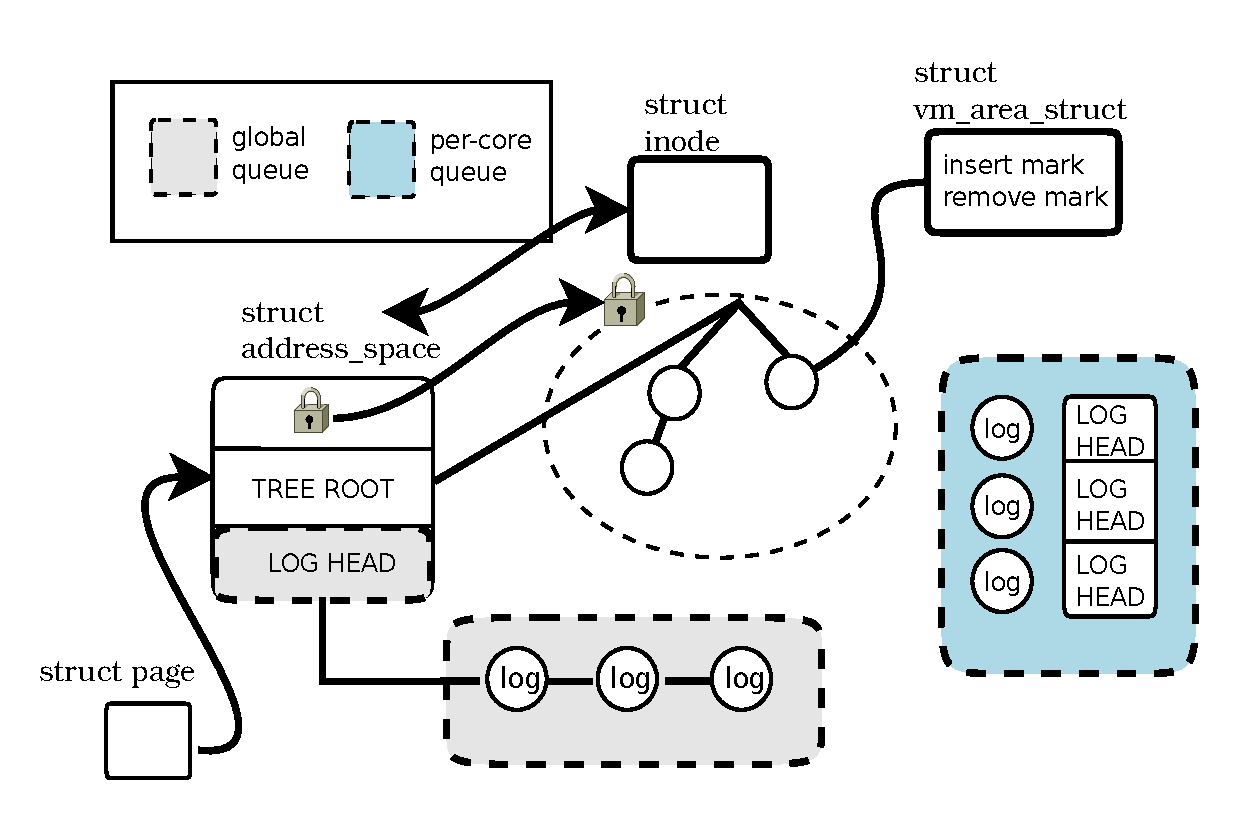
\includegraphics[width=1\textwidth,height=1\textheight,keepaspectratio]{fig/file_rmap}
  \end{center}
  \caption{리눅스 파일 역 매핑에 LDU를 적용한 그림.}
  \label{fig:fileramp}
\end{figure}

%$$$$$$$$$$$$$$$$$$$$$$$$$$$$$$$$$$$$$$$$$$$$$$$$$$$$$$$$$$$$$$$$$$$$$$$$$$$$$$$$
%Paragraph 1: linux의 file mapped page reverse mapping의 구조에 대한 설명
%$$$$$$$$$$$$$$$$$$$$$$$$$$$$$$$$$$$$$$$$$$$$$$$$$$$$$$$$$$$$$$$$$$$$$$$$$$$$$$$$
%Figure \ref{fig:fileramp} shows the rmap for file.
그림 \ref{fig:fileramp}는 파일에 대한 rmap을 보여준다.
%In order to translate physical addresses to virtual address, the
% page(\code{struct page}) indicates the address space object(\code{struct address\_space}), and
%the address space object manages the VMAs by using the
%interval tree.
물리적 주소를 가상 주소로 변경하기 위해서, 페이지는
 address space 오브젝트(\code{struct address\_space})
를 가리키며, address space 오브젝트는 인터벌 트리를 이용하여 VMAs를 관리한다.
%This interval tree is a shared resource between processes.
이러한 인터벌 트리는 프로세스간 공유하는 자원이다. 
%, so Linux kernel uses the reader-writer semaphore to protect the tree.
%Because the system calls such as \code{fork()}, \code{exit()} and
%\code{mmap()} entail concurrent updating VMAs into the shared resource.
\code{fork()} 그리고 \code{exit()}과 같은 시스템 콜은 VMAs에 대해서 동시적 업데이트를 
수반하므로, 프로세스들이 동시에 많은 시스템 콜을 호출할 때, 파일 ramp은 업데이트 명령어 때문에
직렬화가 된다. 
%when the processes simultaneously invoke these system calls, the
%file rmap can be serialized at the update operations.

%$$$$$$$$$$$$$$$$$$$$$$$$$$$$$$$$$$$$$$$$$$$$$$$$$$$$$$$$$$$$$$$$$$$$$$$$$$$$$$$$
%Paragraph 2: file mapping에 ldu 적용한 방법에 대한 설명 
%$$$$$$$$$$$$$$$$$$$$$$$$$$$$$$$$$$$$$$$$$$$$$$$$$$$$$$$$$$$$$$$$$$$$$$$$$$$$$$$$
%The \LDU can easily be applied to the file ramp data structure.
LDU는 파일 rmap 자료구조에 쉽게 적용될 수 있다. 
%For instance, to use the \LDU, a developer adds log's queue header into the
% per-core memory or into the original data structure(\code{struct address\_space}), and
%then adds mark field to the individual object(\code{struct vm\_area\_struct}).
예를 들어, LDU를 사용하기 위해서는 개발자는 로그의 큐 헤더를 퍼코어 메모리에 저장하던지, 아니면 
원본 자료구조(\code{struct address\_space})에 저장하면 된다. 그리고 각각의 오브젝트(\code{struct
vm\_area\_struct})에 마크필드를 추가하면 된다. 

%Then, the developer modifies update function to logging function without a
% lock.
그리고 개발자는 락 없이 업데이트 함수를 로깅 함수로 수정한다.  
%Finally, the developer creates \code{synchronize} function and calls
%the \code{synchronize} function before the read.
마지막으로 개발자는  \code{synchronize} 함수를 만들고, 이것을 리드 전에 호출되도록 수정한다.
%the mark field adds to the individual object(\code{struct
%vm\_area\_struct}), and then the log's queue is added into the per-core
%memory or the global head object(\code{struct address\_space}).

%This figure clearly shows why the \LDU additionally supports the
%global queue because it is a simpler and easier scheme because the log's head
%pointer is located in the interval tree's data structure.
이 그림은 왜 LDU가 추가적으로 전역 큐를 사용하는지를 보여준다. 
이것은 로그의 헤드 포인터가 인터벌 트리의 자료구조에 위치하기 때문이다.
반면에, 퍼코어 큐는 헤드에 대한 메모리의 위치가 다르므로,  
추가적인 퍼코어 큐에 대한 관리 방법이 필요하다. 
%On the other hand, the
%per-core queue may need an additional per-core queue management scheme due
%to the its isolated memory location.



\begin{figure*}[h]
\begin{center}
\inputminted[linenos,fontsize=\footnotesize,
tabsize=4]{c}{src/ldu_queue_global.c}
\end{center}
%\rule{\columnwidth}{0.5pt}
%\vspace{-\baselineskip}
\caption{LDU의 전역 큐.}
\label{fig:glduphysicalupdate}
\end{figure*}

\subsection{자세한 구현 내용}
%$$$$$$$$$$$$$$$$$$$$$$$$$$$$$$$$$$$$$$$$$$$$$$$$$$$$$$$$$$$$$$$$$$$$$$$$$$$$$$$$
%Paragraph 2: per-core queue 구현에 대한 설명 
%$$$$$$$$$$$$$$$$$$$$$$$$$$$$$$$$$$$$$$$$$$$$$$$$$$$$$$$$$$$$$$$$$$$$$$$$$$$$$$$$
%Because the log's head pointer for the per-core queue is
%separated with the original data structure, the implementation of
%per-core queue uses 
%a per-core hash table method that can allow each object to distinguish.
퍼코어 큐를 위한 로그의 헤드 포인트 위치가 큐는 원본 자료구조와 분리 되어 있으므로, 
퍼코어 큐의 구현은 퍼코어 해시 테이블(per-core hash table) 방법을 이용하였다. 이것은
각각의 오브젝트들을 구분 할 수 있게 해준다.
%The per-core hash table implemented as a direct-mapped cache, which one
%bucket only has an object because recently used objects will be in the hash
%table in a way similar to the OpLog's per-core hash table.
퍼코어 해쉬 테이블은 직접 사상 캐시(direct-mapped cache)를 구현하였다. 이것은 하나의
 해시 버켓(bucket)에는 오직 하나의 오브젝트만 존재하는 방법이다.
그 이유는 최근에 사용된 오브젝트가 다시 사용될 활률이 크기 때문이며, 이것은 OpLog의 
퍼코어 해시 테이블 방법과 비슷하다.
%When this hash table is met a hash conflict, the \LDU evicts the object in the
%hash slot.
만약 해쉬 테이블이 충돌을 만나면, LDU는 충돌난 오브젝트를 해쉬 슬롯에서 부터 내보낸다.
%Moreover, this method reduces additional tasks of programmers because it can
%minimize code modifications and does not need an additional lock.
더욱이, 이러한 방법은 프로그래머의 추가적인 작업을 줄인다. 
그 이유는 이것은 코드의 수정을 최소화할 수 있고 추가적인 락이 필요가 없기 때문이다.
%The per-core hash table, however, incurs a hash conflict overhead.
하지만 퍼코어 해시 테이블은 해시 충돌에 따른 오버헤드를 낳는다.
%This method is useful when a number of the root objects are infrequently
% created like the file rmap(\code{struct address\_space}).
이러한 방법은 파일 rmap(\code{struct address\_space})과 같이
 작은 빈도수로 루트 오브젝트가 생성될 때 효율적이다. 
%On the other hand, since the anonymous rmap severely creates many
%root objects(\code{struct anon\_vma}), it causes a hash conflict overhead.
반면에, 익명 ramp은 극심하게 루트 오브젝트((\code{struct anon\_vma})들을 생성하기 때문에, 
이것은 심한 해쉬 충돌 오버헤드를 발생한다. 
%Therefore, in the case of the anonymous ramp, we did not distinguish object
%headers, but it needs additional tasks with global lock.
그러므로, 익명 rmap과 같은 경우에는 우리는 오브젝트의 헤더를 구별하지 않았다. 
그러나 이것은 추가적인 프로그래머의 작업과 전역 락이 필요하다.



\begin{figure}[h!]
\begin{center}
\inputminted[linenos,fontsize=\footnotesize,
tabsize=4]{c}{src/ldu_queue_per_core.c}
\end{center}
%\rule{\columnwidth}{0.5pt}
%\vspace{-\baselineskip}
\caption{LDU의 퍼코어 큐.}
\label{fig:glduphysicalupdate}
\end{figure}





%$$$$$$$$$$$$$$$$$$$$$$$$$$$$$$$$$$$$$$$$$$$$$$$$$$$$$$$$$$$$$$$$$$$$$$$$$$$$$$$$
%Paragraph 1: 커널 버전 및 코드 분량, 테스트에 대한 설명
%$$$$$$$$$$$$$$$$$$$$$$$$$$$$$$$$$$$$$$$$$$$$$$$$$$$$$$$$$$$$$$$$$$$$$$$$$$$$$$$$
%We have implemented the new deferred update algorithm in Linux 4.5-rc6 kernel,
%and our modified Linux is available as open source. 
우리는 새로운 지연 업데이트 알고르즘을 리눅스 4.5-rc6 커널에 구현하였고, 우리의 
수정된 리눅스는 오픈소스로 이용할 수 있다.  
%The version of global queue modified code is xx that less complex, but per-core
%queue the modified code is xx-xx.
%The implementation is stable enough and has passed the testing
%related with virtual memory, scheduler,
%and file in the Linux Test Project~\cite{LTP}.
우리의 구현은 충분히 안정적이며, 리눅스의 테스트 프로젝트(Linux Test Project)~\cite{LTP}
 중에서 가상 메모리, 스케줄러 그리고 파일과 관련된 테스트를 모두 통과하였다. 
